\chapter{Implementation}
\label{chapter:implementation}

The implementation chapter contains a description of the different attempted dead reckoning approaches and the required constraints.
Thereafter, an overview and implementation of different classes is shown.
Finally, precision tests is analysed, in order to determine how accurate the implemented dead reckoning technique is.

\section{Dead Reckoning Approaches}\label{section:dead-reckoning-approaches}
%Meta
When implementing dead reckoning techniques, various approaches were attempted, which had different strengths and weaknesses.
It proved to be a good learning experience, as it indicated what considerations were key to implement dead reckoning.

%KUN areal - pege tilbage til teori
% + nem, løbende udregninger
% - upræcist, tog ikke højde for støj'
\subsection*{Initial Approach}
The initial approach was primarily based on the theory in \secref{sec:position-calculations}, which explained the relation between acceleration, velocity, and position. 
It was done with an algorithm that recorded all accelerations.
The algorithm used these values to calculate the velocity and the user's estimated position. 
This approach was simple but suffered from noise, as the noise would also change the velocity and thus the position, without the user actually moving.

%Inddeling i skridt, areal + filtrering.
% + mere præcist
% - stadig upræcist, ikke løbende udregninger, kompliceret.
\subsection*{Filters}
To reduce the noise impact on the position, a filter was implemented, see \secref{subsection:exponential-moving-average}. 
It proved to be a fast and simple approach to reduce the noise impact.
In order to prevent noise from having an impact on the position, when the user is not moving, an algorithm was developed.
This approach hindered the algorithm from registering the position change, as it would only change the position once a complete step was taken.

Another hindrance for the algorithm was when taking many steps to one side.
Which rendered the algorithm unable to determine whether a step was to the left or to the right, as the steps were done with too high frequency. 
For that reason, this algorithm was deemed undesirable as the intention of the algorithm was to be used in games, which requires a fast update.
However, it would not have been a concern if updating the position during a step was not necessary.

%Areal, med constraints og filtrering
% + nem, præcist, løbende udregninger
% - ikke så robust, tog ikke højde for tyngdeacceleration
\subsection*{Constraints}
With the previous approaches in mind, another algorithm was made, which had the same general idea of calculating the position with the theory from \secref{sec:position-calculations}.
A calibration was done to filter out the acceleration offset noise. 

Furthermore, when developing an algorithm with this approach, different constraints were added, to cancel out any undesired position-estimation updates.
One constraint was setting a limit on the area a user was allowed to move within. 
In the case where the user was estimated to be beyond this area, the position was set to the edge of the area.
 
Another constraint was that if the acceleration was too low, it would be discarded.
This acceleration was discarded since it would give a change in position when a step was not performed. 
In addition, if the acceleration was under a specific limit for too long, the velocity was set to zero, as it was interpreted to the user standing still.
Although this algorithm took noise into account, and the position accuracy was improved.
A problem remained, if the phone was tilted as the gravitational pull would have an impact on the acceleration registered.
Finally, whenever a step was taken, the deceleration would make the estimated position move backwards, since the deceleration was bigger than the corresponding acceleration, resulting in a velocity with opposite direction.

In order to take the gravitational pull into account, the \textit{Motion} class from Microsoft \citep{misc:motionclass} was tested.
The class used the accelerometer in conjunction with the gyroscope and the magnetometer to cancel out the gravitational pull.
This seemed as an easy way to accomplish the goal.
However, it was unclear how the Motion class altered the data, and for that reason it was not used further.

\subsection*{Bayesian Structure}
With these approaches in mind, a dynamic Bayesian network was modelled.
It proved to give a good overview of the different calculations needed to determine the user's position.
In addition, the marginal probability distribution for each stochastic variable was found by use of the theory from \secref{section:normal-distribution}.
The variance, found when determining the marginal probability distribution, was not used, since no observations were used. 
However, by calculating the variance, with observations on the position nodes, the network would be an extended Kalman filter.
The variance would then have an influence on the mean of the marginal probability distribution of the position, as described in \secref{section:insert-evidence}.

\subsection*{Corrected Moving Average}
A problem found was the velocity gain, because of the deceleration being larger than the acceleration, resulting in the velocity being in the opposite direction than what was performed.
This problem was solved by adjusting the deceleration to be the same as the acceleration with opposite direction. 
The adjustment was a hack in the Bayesian network, as the mean value for the deceleration nodes were assigned to be the same but in the opposite direction of the accelerations of the step. 
The adjustment is different from the direct combination approach, as described in \secref{section:direct-combination}, and therefore it is a hack.
By implementing this hack, the velocity gain problem was corrected, but resulted in a limitation of how fast a user could take steps.
It was deemed to not being a problem, as the game became playable, with the constraint in mind.

\subsection*{Rotation}
With the correction of the deceleration problem, another problem still existed, which was accidental phone-rotation when moving.
To correct for pitch-rotation, the magnetometer of the phone was first used to determine the angle of the pitch-rotation.
This angle would then be used in conjunction with trigonometry to correct the acceleration when moving.

The yaw-rotation had to be taken into account, as the gravitational pull would affect the measured acceleration.
In order to correct for gravitational pull, the gyroscope was used in conjunction with the accelerometer to determine the yaw-rotation angle.
The gyroscope would, over time, drift and make the angle inaccurate.
To avoid drifting, a complementary filter was implemented.
The complementary filter used the angles determined by accumulating the gyroscope readings, as well as determining the angle by use of the accelerometer readings.

With the correction of the gravitation pull implemented, it was found that the gyroscope and accelerometer approach was better than using the compass for this application.
Therefore, the gyroscope was used to handle both pitch- and yaw-rotation, as the compass was slow to adjust to a new angle, whereas the gyroscope and accelerometer was faster.

After having used these various approaches, four constraints remained. 
These constraints will be explained in more details in the next section.	
\section{Constraints}\label{section:constraints}
The purpose of this section is to describe a set of constraints. 
The reason for doing so, is the limited time allotted for the project. 
The constraints that are applied to the project have each been depicted in \figref{figure:constraints}.
Each constraint is explained below, the letter in the list corresponds to the letter in \figref{figure:constraints}.  

\begin{enumerate}[label=(\alph*),itemsep=2pt,parsep=2pt]
%\item Jitter noise is caused by tiny vibrations and occurs when the player is handling the device.
%Therefore, the application will ignore all gravitational-values between -0.1 g and 0.1 g.
\item To simplify the complexity of the application, the movement-area for the player will be a fixed size of $300 cm$ in width.
It means that the player will have to play within the movement-area.
%\item To help the application decide whether a step is actually a step, the maximum length of a step is limited to 100 cm.
%\item The minimum length of a step is set to 20 cm.
\item To ensure consistency in accelerometer readings, a player must hold the device in landscape mode, with the touch pad buttons to the right and the x-axis in a vertical line. As it is impossible to keep the phone completely steady while moving, the application will allow for a rotation of up to $30^\circ$ around the x- and z-axis.
\item The maximum velocity is limited to $3 m/s$, as the player should not be able to move faster than this.
\item Acceleration is constrained to $1 g$. From observations, accelerations with a value exceeding $1 g$ does not happen while side stepping, this includes both negative and positive acceleration values.
\end{enumerate}

\begin{figure}[h]
	\centering
	%---- linebreak	
	\begin{subfigure}[b]{0.45\textwidth}
		\centering
		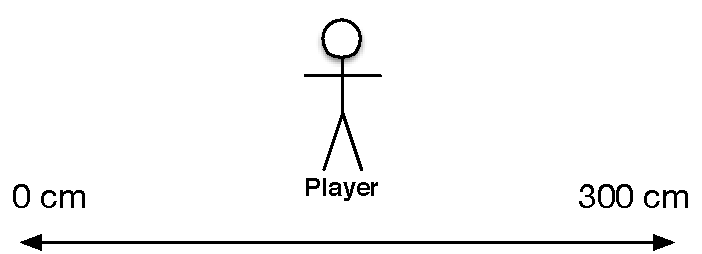
\includegraphics[scale = 0.45]{media/constraints/02-fixed-movement-area}
		\caption{Fixed movement area.}
		\label{figure:fixed-movement-area}
	\end{subfigure}
	\qquad
	\begin{subfigure}[b]{0.45\textwidth}
		\centering
		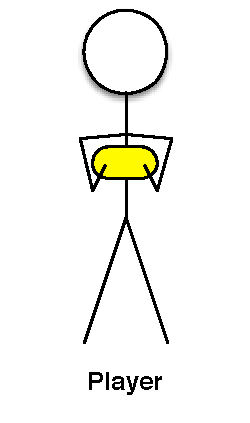
\includegraphics[scale = 0.45]{media/constraints/05-fixed-device-position}
		\caption{Fixed device position.}
		\label{figure:fixed-device-position}
	\end{subfigure}
	%---- linebreak
	\begin{subfigure}[b]{0.45\textwidth}
		\centering
		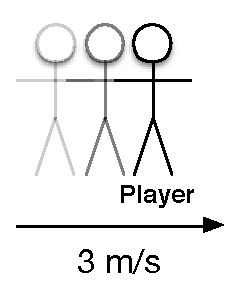
\includegraphics[scale = 0.45]{media/constraints/06-maximum-velocity}
		\caption{Maximum velocity.}
		\label{figure:maximum-velocity}
	\end{subfigure}
	\qquad
	\begin{subfigure}[b]{0.45\textwidth}
		\centering
		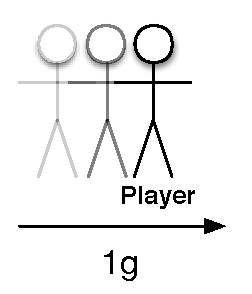
\includegraphics[scale = 0.45]{media/constraints/07-maximum-acceleration}
		\caption{Maximum acceleration.}
		\label{figure:maximum-gravitational-pull}
	\end{subfigure}		
	\caption{Constraints}
	\label{figure:constraints}
\end{figure}
\section{Class diagram}
In this section, the class diagram of the dynamic Bayesian network, see \figref{figure:class-diagram}, will be shown and explained, to give an overview of the structure of the Bayesian network implementation.

\begin{figure}[H]
     \centering
     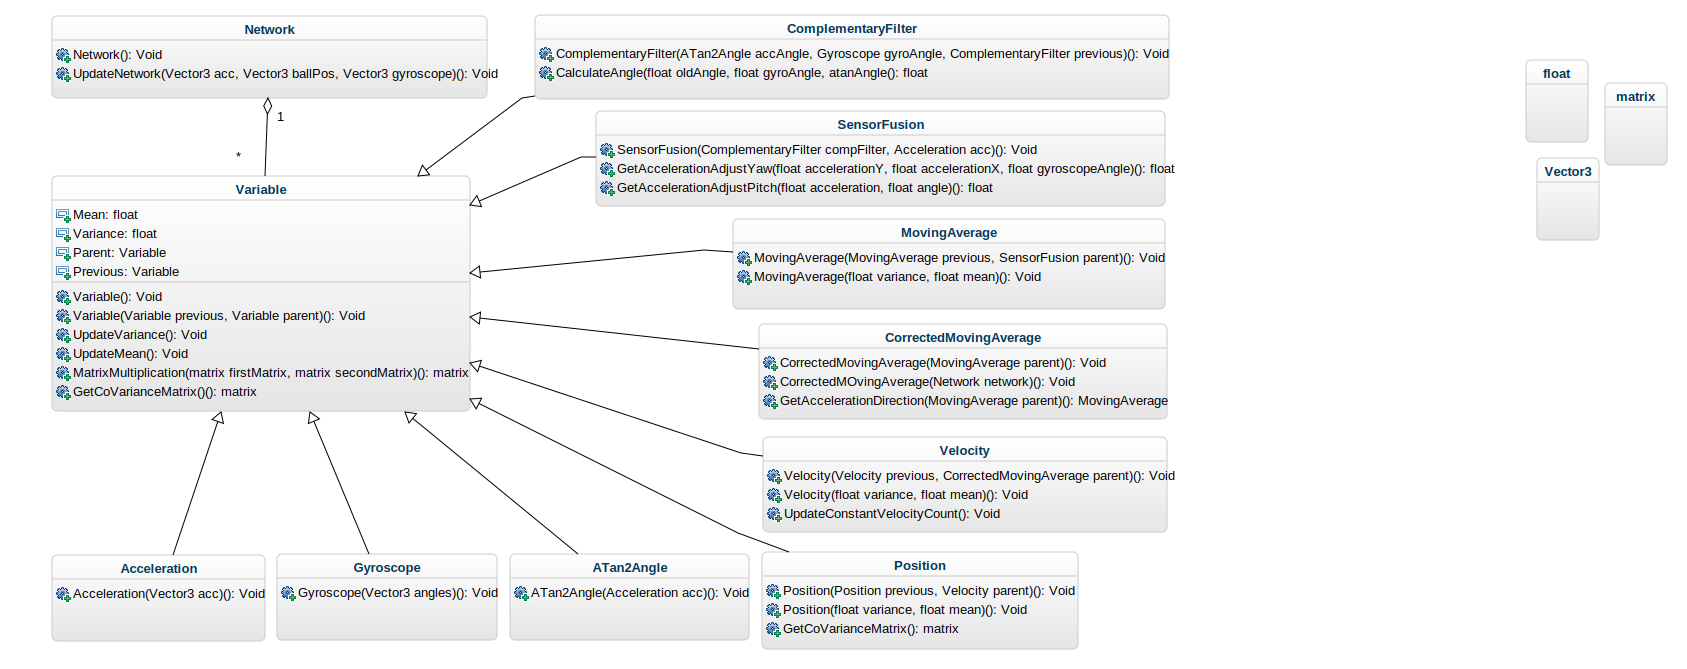
\includegraphics[trim=0cm 0cm 5cm 0cm,clip,scale=1.25]{implementation/classdiagramb}
     \caption{Class diagram for developed navigation library.}     
     \label{figure:class-diagram}
\end{figure}

To implement a dynamic Bayesian network, the structure from \figref{figure:class-diagram} was used.
The \textit{Network} class keeps track of the overall structure of the dynamic Bayesian network.
In order to keep track of the structure, the \textit{Variable} class has nine subclasses.
The Variable class exists to calculate the marginal probability distribution for each of its subclasses.
Each subclass then calculates the concrete probability distribution and constraints, which varies for each of the subclasses.

Concrete implementation of a sample of the classes in \figref{figure:class-diagram} will be described in the next sections.
\input{content/implementation/network}
\section{Acceleration}
Acceleration is a class implemented to represent the $Acc$ node from the Bayesian network. It inherits from the abstract Variable class, where the Variable class serves as a structure that all nodes in the network must have.

Since Acceleration inherits from Variable it has to implement two methods, \lstinline$UpdateVariance$ and \lstinline$UpdateMean$.
The mean value is the accelerometer reading.
The variance for the acceleration is a constant value and is determined by testing, which is described in \secref{section:finding-the-variance}.
Furthermore, when inheriting from Variable a matrix multiplication method is provided, as well as four properties, keeping track of a stochastic variable's mean, variance, and its parents.

The readings from the accelerometer were uncertain, as of such, the variance for the accelerometer readings was determined, which is described hereafter.

\subsection{Finding the Variance}\label{section:finding-the-variance}
To measure the distribution of noise from the accelerometer, the formula for finding variance, as shown in \secref{section:normal-distribution}, will be utilised.
The device was placed on a flat surface for a period of three minutes, to record a set of accelerations containing noise.
This data was used to calculate $\mu$, which is the mean value for the stochastic variable $X$.
The expected value would be zero, as the device was not in motion when the data was recorded.
The following formula was used to approximate the mean acceleration:

\begin{equation*}
\mu = \frac{1}{n}\sum\limits_{i=1}^n\left(X_i\right)
\end{equation*}
 	
where, $n$ is the amount of data entries and $X_i$ is the $i$'th entry.
For the chosen device, the mean value was calculated to $\textbf{0.00026 g}$.
When the mean value is known, it can be used to approximate $\sigma^2$, which is the variance which can be approximated as follows:

\begin{equation*}
\sigma^2 = \frac{1}{n}\sum\limits_{i=1}^{n}\left( X_i - \mu \right)^2
\end{equation*}

where, $n$ is the amount of data entries, $X_i$ is the $i$'th entry, and $\mu$ is the mean value.
For the chosen device, the variance was calculated to $\textbf{0.00552 g}$.

By finding the mean value and the variance, a normal distribution can be implemented on measured accelerations by using the \eqref{eq:normaldist} as repeated below:

\begin{equation*}
f(x) = \frac{1}{\sigma \sqrt{2\pi}}e^{-\frac{(x - \mu)^2}{2 * \sigma^2}}
\end{equation*}

\figref{fig:finding-the-variance-chart} shows the final result of finding the normal distribution.
The red points plotted in the graph, is the amount of times the specific value has been recorded during the three minutes of recording.
The blue graph shows the normal distribution which has been calculated from the recorded values.
It can be seen that the red points and blue graph are not aligned.
However, it is not an issue, since the ordinate axis specifies amount and density for the red points and blue graph respectively.

\begin{figure}[h]
\centering
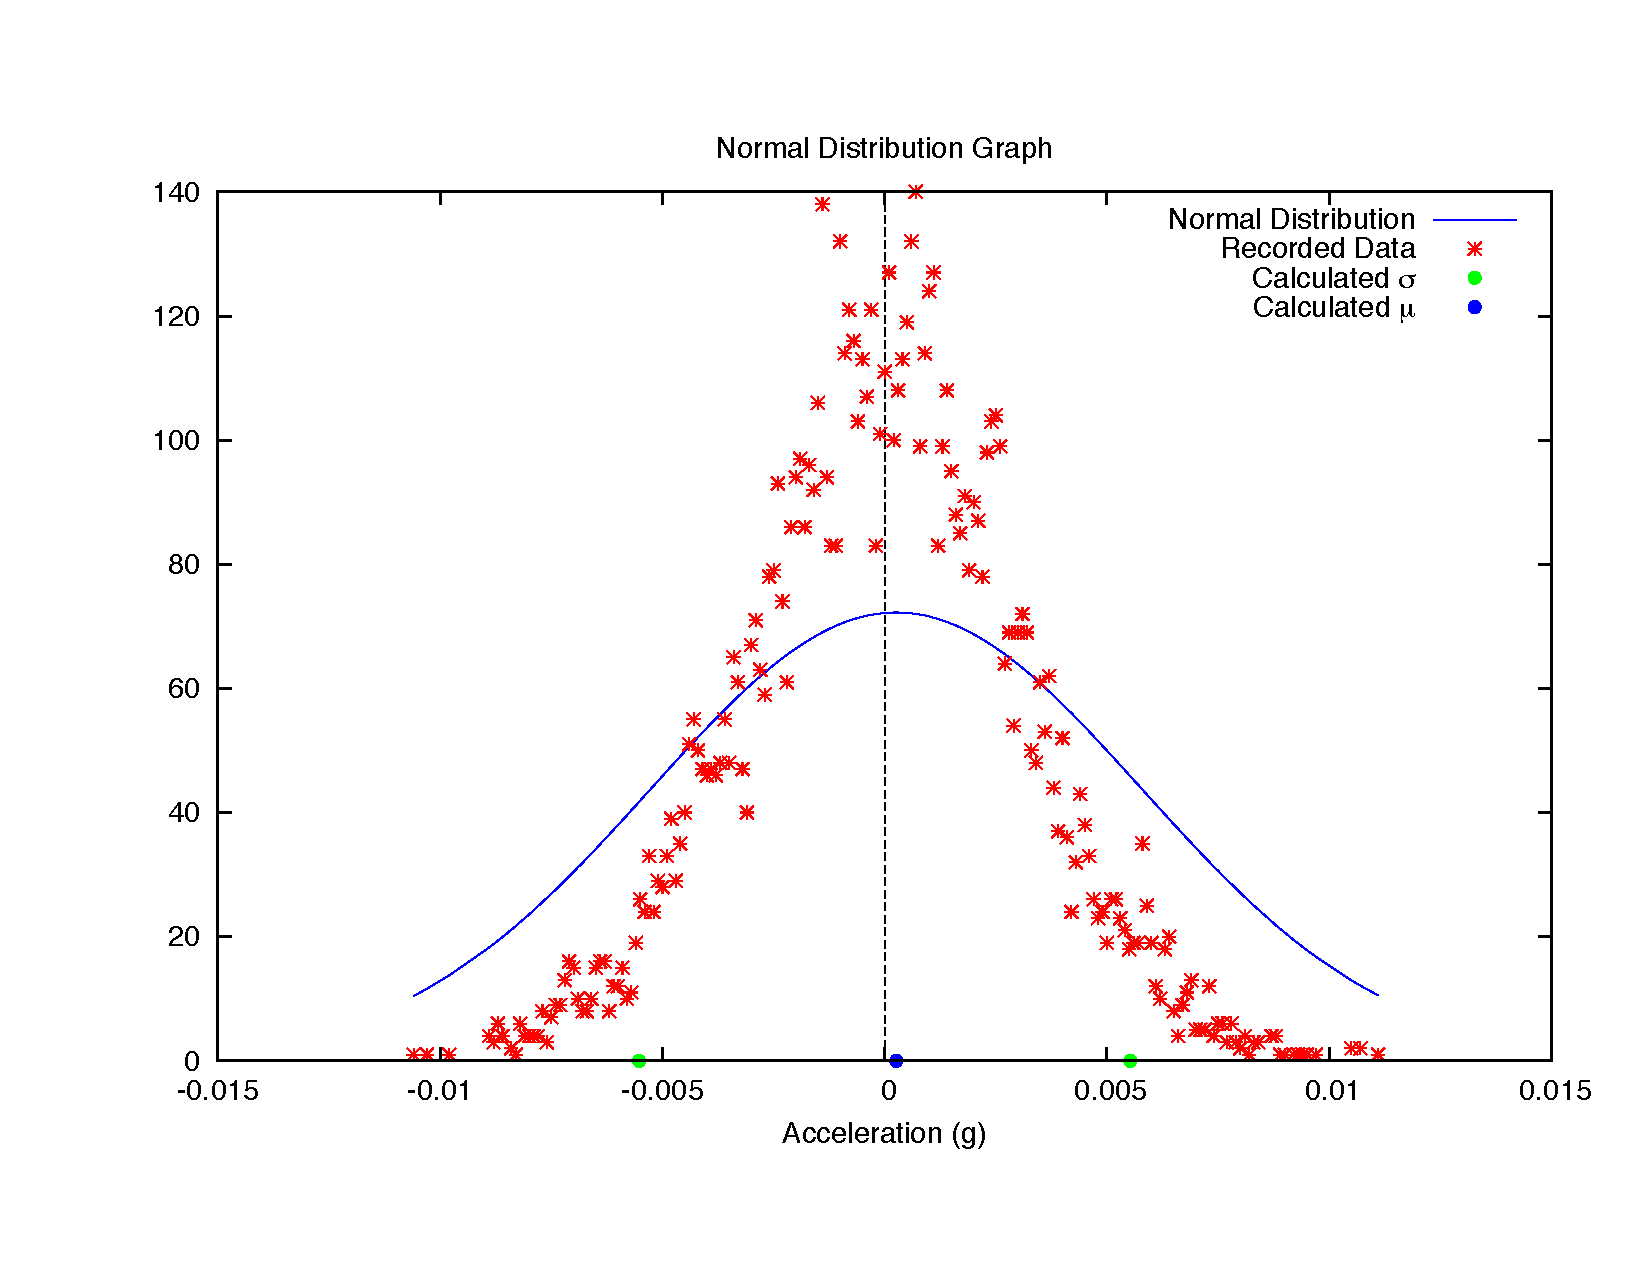
\includegraphics[trim = 0cm 2cm 0cm 2cm, clip, scale=0.45]{media/gnuplot/normaldist.pdf}
\caption{Finding $\mu$, $\sigma$, and the normal distribution}
\label{fig:finding-the-variance-chart}
\end{figure}

\section{SensorFusion}\label{section:SensorFusion}
The \textit{SensorFusion} class is implemented to adjust for yaw and pitch-rotations, where the yaw and pitch-rotation angles are provided in the constructor.
The SensorFusion adjusts the acceleration readings in the y-axis in two methods.


The method in \lstref{lst:acceleration-yaw} corrects the acceleration when the phone is tilted around the z-axis, and is important since it is affected by the gravitational pull.

When the yaw-rotation has been found, using the accelerometer and gyroscope, the gravitational pull is taken into account. 
The method, seen in \lstref{lst:acceleration-yaw}, calculates movement acceleration, without gravitational pull, is found using trigonometry.

\begin{lstlisting}[caption={Method correcting acceleration when tilted around the z-axis.}, label=lst:acceleration-yaw, float=h, style=sharpc]
private float GetAccelerationAdjustYaw(float accelerationY, float accelerationX, float gyroscopeAngle)
{
	return (float)((accelerationY - (-accelerationX * Math.Sin(gyroscopeAngle))) / (Math.Cos(gyroscopeAngle)));
}
\end{lstlisting}

An illustration of the gravitational pull problem can be seen in \figref{figure:yaw-rotation-adjustment}, which is used to explain \lstref{lst:acceleration-yaw}.

\begin{figure}[H]
	\centering
	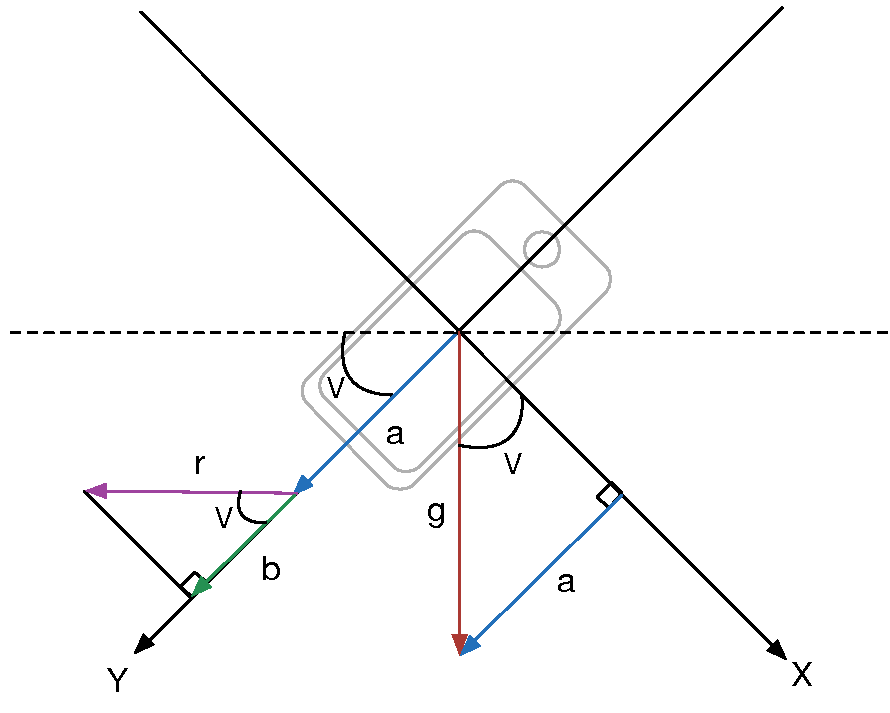
\includegraphics[trim = 0cm 0cm 0cm 3cm, clip, scale=0.75]{media/graph}
	\caption{Yaw-rotation adjustment.}
	\label{figure:yaw-rotation-adjustment}
\end{figure}

In \figref{figure:yaw-rotation-adjustment}, the phone is tilted in an angle of $V$.
$r$ is the desired acceleration, as it is the acceleration, in the y-axis, without gravitational pull. 
$a + b$, is the measured acceleration in the y-axis of the accelerometer.
$g$ is the gravitational pull, which is constant.
$g$ is used in combination with the angle $V$ to calculate $a$, which is how much the gravitational pull affects the measured acceleration in the y-axis.

\begin{equation}\label{equation:vector-a}\centering
a = g \cdot sin(V)
\end{equation}

Once $a$ has been found, using \eqref{equation:vector-a}, $b$ can be found by subtracting $a$ from the measured acceleration in the y-axis.
$b$ is the acceleration in the y-axis, unaffected by gravitational pull, however, the desired acceleration is in the horizontal plane.
As of such, $V$ and $b$, is used to find $r$, seen in \eqref{equation:vector-r}.

\begin{equation}\label{equation:vector-r}\centering
    r = \frac{b}{cos(V)}
\end{equation}

The measured acceleration in the y-axis, $m_{acc}$, is given by $a + b$.
Hence, the final formula for finding $r$ is \eqref{equation:vector-final}.

\begin{equation}\label{equation:vector-final}\centering
    r = \frac{m_{acc} - g \cdot sin(V)}{cos(V)}
\end{equation}

Much like the adjustment in the yaw-rotation, a similar correction is performed for pitch-rotation. 
However, for pitch-rotation there is no gravitational pull affecting the measured acceleration. 
For that reason, it is sufficient to use \eqref{equation:vector-r}, as $b$ is the measured acceleration.
This correction has to be calculated after the correction of the yaw-rotation.  

\begin{lstlisting}[caption={Method correcting acceleration when tilted around the x-axis.}, label=lst:acceleration-pitch, float=h, style=sharpc]
private float GetAccelerationAdjustPitch(float acceleration, float angle)
{
	return acceleration / (float)Math.Cos(angle);
}
\end{lstlisting}

The calculation of the marginal probability distribution of the SensorFusion node is not done with a direct combination.
For that reason, the variance can not be determined as the marginal distribution of the nodes that are constructed with a direct combination.
Although, the current implementation of calculating the variance of the SensorFusion node as the sum of the variance of the parents is not correct, it is done since a better solution was not present.
\section{CorrectedMovingAverage}
The \textit{CorrectedMovingAverage} class adjusts the acceleration, such that a deceleration of a step is the same size as the acceleration of the step.
This adjustment is done with the help of a stack which saves each step of an acceleration, such that it can be used for the corresponding deceleration.
As mentioned in \secref{section:dead-reckoning-approaches}, it is a hack, since it does not follow the defined rules for updating the marginal probability distributions.
However, it proved to be a good solution that takes the velocity gain into account.

To track the direction of a step, an enumerator was created which had the elements \textit{Unknown}, \textit{Left}, and \textit{Right}. 
When the step direction is unknown, a step has not been detected yet and the program checks each acceleration to see if it is outside the jitter zone.
Jitter noise occurs when the user unintentionally shakes the phone.
The jitter zone is an interval specifying where jitter noise can occur.
When the acceleration is higher than the jitter zone, a right step has begun, and if it is lower, it is a left step.
This categorisation is done with the knowledge of how an acceleration graph for a step is shaped, and is found in \secref{section:accelerometer}.
In addition, when a step has been detected, the velocity is reset to zero as the step has just begun.

If a step is in progress, every next acceleration, which is in the same direction, is loaded into a stack.
Once the deceleration has begun, the stack is popped for each consecutive deceleration.

\section{Position}
The \textit{Position} class is used to track the position of the phone, and is a subclass of the Variable class.
The position has three parents, which is the previous position, current velocity, and the ball position corresponding to the dynamic Bayesian network described in \secref{section:dynamic-bayesian-network}.

\begin{lstlisting}[caption={Update mean method containing constraints for position}, label=lst:PositionConstraint, float=h, style=sharpc]
protected override void UpdateMean()
{
    Mean = Constants.POSITION_MEAN_GAIN + Constants.F_POSITION[0, 0] * Parent.Mean + Constants.F_POSITION[0, 1] * Previous.Mean;

    if (Mean > Constants.POSITION_MAX || Mean < Constants.POSITION_MIN)
    {
        if (Mean > Constants.POSITION_MAX)
            Mean = Constants.POSITION_MAX;
        else
            Mean = Constants.POSITION_MIN;    
        
        Variance = 0.0f;
        Parent.Mean = 0.0f;
        Parent.Variance = 0.0f;
    }
}
\end{lstlisting}

In \lstref{lst:PositionConstraint}, the \lstinline$UpdateMean$ method has been implemented to take all parents into account for the Mean, as can be seen on line 3.
However, a constraint on the mean of the position has also been implemented, which is the limit of the area, corresponding to walking into the wall, see \figref{figure:fixed-movement-area} and can be seen in line 5.
The constraint resets the variance of the position in line 12, and resets the mean and variance of the velocity in line 13-14, and is implemented to handle uncertainties in the positioning measurement.
\section{Precision Test}
Once the application was developed, the datalogger was used to gather new data such that a precision test could be performed.
Data was recorded in distances of $1$, $2$, $25$, and $50$ meters.
These data were used to determine the correctness of the output given by the application.

Tables showing the test results can be seen in \appref{app:precision-tests}.
The majority of the tests showed that the application underestimated the calculated positions and the average calculated position was $46.1\%$ of the actual position.
The percent deviation ranged from $22.8\%$ to $164.1\%$, however, only $6$ calculated positions were above $70\%$ while $81$ were below $70\%$.
To summarize the percent deviation, a bar chart was made to show an overview of the data, see \figref{figure:acc-histo}.
%Hamuns ekstra edit End:

Various reasons for this underestimation could be the filters suppressing the accelerations, the rotation of the phone still having affect on the accelerations, or that the sensor readings in general measure too low values.

This underestimation could be corrected in various ways.
One way could be to scale the position with a factor, or to make further adjustments in the actual implementation.
Some of these adjustments are discussed in \chapref{chapter:discussion}.

\begin{figure}[H]
	\centering
	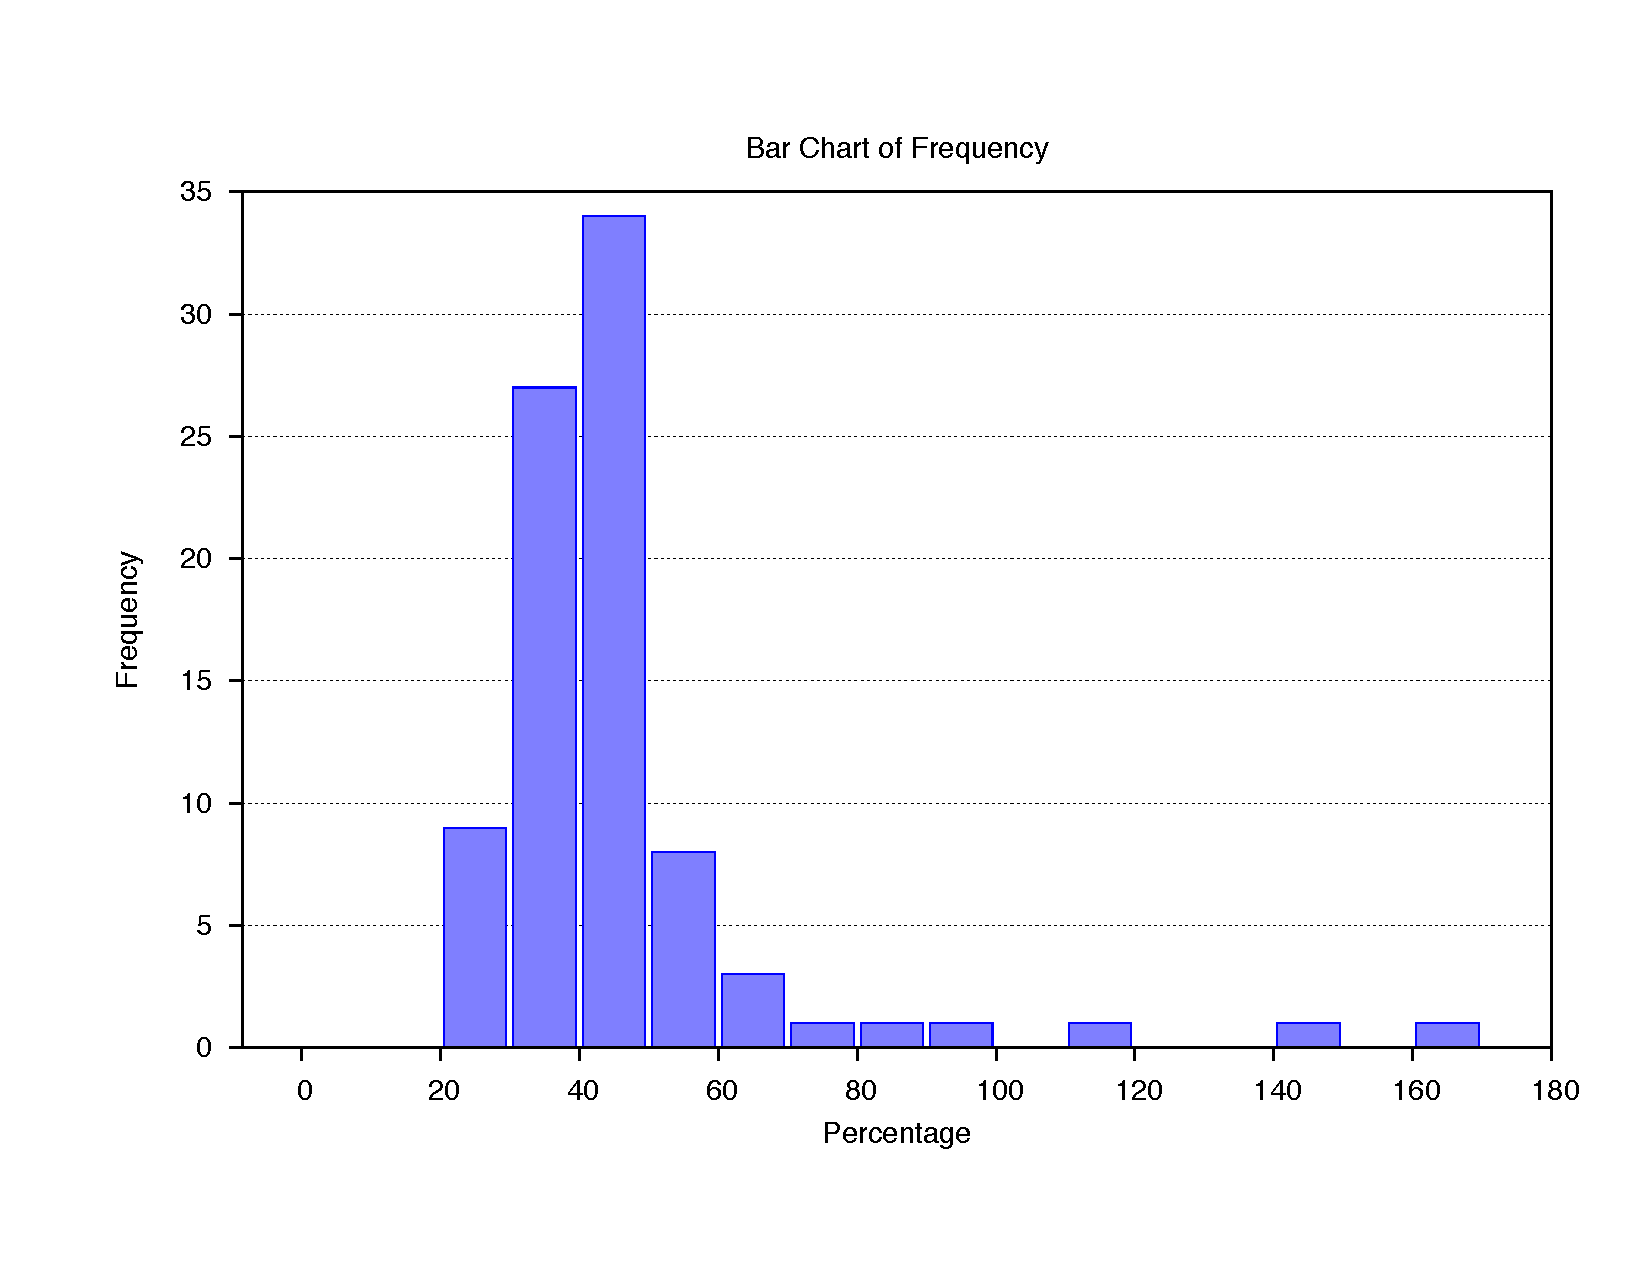
\includegraphics[scale=0.5, trim = 0cm 2cm 0cm 2cm, clip]{media/gnuplot/barchart.pdf}
	\caption{A bar chart for the percent deviation range and how many times it has been observed.}
	\label{figure:acc-histo}
\end{figure}
